\chapter{METODE PENELITIAN}

\section{Jenis Penelitian}
Penelitian ini mengadopsi pendekatan penelitian terapan, dengan fokus utama pada implementasi teknologi Hybrid Modeling dalam pengembangan sistem rekomendasi topik skripsi. Melalui pendekatan ini, penelitian bertujuan untuk mengaplikasikan dan mengevaluasi efektivitas metode Hybrid Modeling dalam konteks spesifik rekomendasi topik skripsi. Alur metode ini dapat dilihat pada Gambar \ref{fig:crisp-dm-overview}

\begin{figure}[H]
    \centering
    \fbox{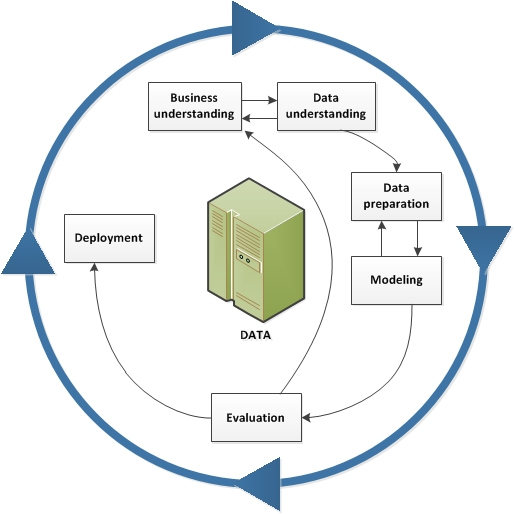
\includegraphics[width=0.55\textwidth]{images/crisp-dm-overview.jpg}}
    \caption{Alur Metode CRISP-DM (IBM, \cite{IBM2022})}
    \label{fig:crisp-dm-overview}
\end{figure}

\section{Waktu dan Tempat Penelitian}
% TODO: Sesuaikan detail spesifik
Penelitian ini dilaksanakan dalam rentang waktu empat bulan, dimulai dari Agustus 2024 hingga November 2024. Pengumpulan data dilakukan melalui akuisisi dataset dari Program Studi ..., yang menyediakan basis data komprehensif mengenai topik-topik skripsi yang telah diajukan sebelumnya.

\section{Sarana dan Pendukung}
Untuk memastikan keberhasilan dan efisiensi penelitian ini, berbagai sarana pendukung telah diidentifikasi dan disiapkan. Perangkat keras dan perangkat lunak yang dipilih tidak hanya mendukung pelaksanaan penelitian, tetapi juga memungkinkan pengembangan dan pengujian sistem rekomendasi secara optimal. Berikut adalah rincian perangkat yang digunakan:

\subsection{Perangkat Keras}
\begin{enumerate}
    \item Memori RAM 8GB DDR3, yang menyediakan kapasitas yang memadai untuk pemrosesan data dan eksekusi model.
    \item Penyimpanan SSD 256GB, memungkinkan akses data yang cepat dan efisien, serta mempercepat proses komputasi.
\end{enumerate}

\subsection{Perangkat Lunak}
\begin{enumerate}
    \item Python versi 3 atau lebih tinggi, dipilih sebagai bahasa pemrograman utama untuk pengembangan dan implementasi model machine learning.
    \item Flask, framework web Python yang ringan dan fleksibel, digunakan untuk mengekspos model sebagai API, memfasilitasi integrasi dengan komponen sistem lainnya.
    \item Node.js, platform JavaScript server-side yang kuat, berfungsi sebagai backend untuk mengelola logika aplikasi dan alur data.
    \item React.js, library JavaScript modern untuk pengembangan antarmuka pengguna, dipilih untuk menciptakan pengalaman pengguna yang responsif dan interaktif.
    \item Figma, alat desain kolaboratif berbasis web, digunakan untuk merancang dan memprototype antarmuka pengguna sistem.
    \item Draw.io (App Diagram), platform pembuatan diagram online, dimanfaatkan untuk merancang dan mendokumentasikan arsitektur sistem melalui diagram UML.
\end{enumerate}

\section{Rancangan Penelitian}
Rancangan penelitian ini disusun secara sistematis untuk memastikan pelaksanaan yang terstruktur dan efektif. Dengan mengadopsi metodologi Cross-Industry Standard Process for Data Mining (CRISP-DM), penelitian ini dibagi menjadi beberapa tahapan kritis yang saling terkait. Setiap tahapan dirancang untuk membangun fondasi bagi tahapan berikutnya, memastikan kesinambungan dalam proses penelitian. Berikut adalah uraian detail dari setiap tahapan:

\subsection{Business Understanding}
Tahap ini berfokus pada pemahaman mendalam tentang kebutuhan dan tantangan dalam proses pemilihan topik skripsi. Melalui wawancara dengan stakeholder akademik, analisis tren penelitian terkini, dan evaluasi sistem yang ada, peneliti akan mengidentifikasi peluang peningkatan dan mendefinisikan tujuan spesifik dari sistem rekomendasi yang akan dikembangkan. Pemahaman ini akan menjadi landasan untuk merancang solusi yang tepat sasaran dan bernilai tinggi bagi pengguna akhir.

\subsection{Data Understanding}
Pada tahap ini, peneliti akan melakukan eksplorasi mendalam terhadap dataset topik skripsi yang tersedia. Aktivitas ini mencakup analisis statistik deskriptif, visualisasi data, dan identifikasi pola atau tren yang mungkin ada dalam data. Pemahaman yang baik tentang karakteristik data, termasuk kualitas, kelengkapan, dan relevansinya, akan membantu dalam merancang strategi preprocessing yang efektif dan pemilihan fitur yang tepat untuk model rekomendasi.

\subsection{Data Preparation}
Tahap persiapan data melibatkan serangkaian proses untuk mengolah data mentah menjadi format yang siap digunakan dalam pemodelan. Kegiatan ini mencakup pembersihan data untuk mengatasi nilai yang hilang atau tidak konsisten, normalisasi atau standarisasi fitur numerik, encoding variabel kategorikal, dan potentially feature engineering untuk menciptakan fitur baru yang lebih informatif. Selain itu, dataset akan dibagi menjadi set pelatihan dan pengujian untuk memfasilitasi evaluasi model yang akurat.

\subsection{Modeling}
Dalam tahap pemodelan, peneliti akan mengimplementasikan pendekatan Hybrid Modeling yang menggabungkan teknik machine learning tradisional dengan metode deep learning. Proses ini melibatkan eksperimen dengan berbagai arsitektur model, tuning hyperparameter, dan validasi silang untuk mengoptimalkan performa. Fokus utama adalah pada pengembangan model yang dapat menangkap kompleksitas hubungan antara karakteristik mahasiswa, tren penelitian, dan kesesuaian topik skripsi.

\subsection{Evaluation}
Evaluasi model akan dilakukan secara komprehensif menggunakan berbagai metrik kinerja seperti akurasi, presisi, recall, dan F1-score. Selain itu, analisis kualitatif terhadap rekomendasi yang dihasilkan akan dilakukan untuk memastikan relevansi dan keberagaman topik yang direkomendasikan. Proses evaluasi ini juga akan mencakup perbandingan dengan baseline model untuk mengukur peningkatan yang dicapai oleh pendekatan Hybrid Modeling.

\subsection{Deployment}
Setelah model final dipilih dan divalidasi, tahap deployment akan fokus pada integrasi model ke dalam sistem aplikasi yang user-friendly. Ini melibatkan pengembangan antarmuka pengguna menggunakan React.js, implementasi backend dengan Node.js, dan penyiapan API menggunakan Flask untuk mengekspos fungsionalitas model. Aspek keamanan, skalabilitas, dan performa sistem akan menjadi pertimbangan utama dalam proses deployment.

\subsection{Feedback}
Tahap akhir penelitian akan melibatkan pengumpulan dan analisis umpan balik dari pengguna sistem. Melalui survei pengguna, analisis log penggunaan, dan wawancara dengan stakeholder, peneliti akan mengidentifikasi area untuk perbaikan dan pengembangan lebih lanjut. Informasi ini akan digunakan untuk merumuskan rekomendasi untuk iterasi dan peningkatan sistem di masa depan, memastikan bahwa sistem rekomendasi topik skripsi terus berkembang sesuai dengan kebutuhan pengguna dan tren penelitian yang dinamis.

\section{Jadwal Penelitian}
Jadwal dan waktu pelaksanaan penelitian ini dapat dilihat pada Tabel \ref{tab:jadwal-penelitian}. 

\begin{table}[htbp]
    \centering
    \setlength{\tabcolsep}{4pt}
    \renewcommand{\arraystretch}{1.2}
    \caption{Jadwal Kegiatan Penelitian}
    \label{tab:jadwal-penelitian}
    \begin{tabular}{|c|p{4cm}|c|c|c|c|}
    \hline
    \multirow{2}{*}{\textbf{No}} & \multirow{2}{*}{\textbf{Kegiatan}} & \multicolumn{4}{c|}{\textbf{Bulan}} \\
    \cline{3-6}
     & & \textbf{Agustus} & \textbf{September} & \textbf{Oktober} & \textbf{November} \\
    \hline
    1. & Studi pustaka & \cellcolor{lightgray} & & & \\
    \hline
    2. & Penerimaan proposal & \cellcolor{lightgray} & \cellcolor{lightgray} & & \\
    \hline
    3. & Pengumpulan dan analisis data & \cellcolor{lightgray} & \cellcolor{lightgray} & & \\
    \hline
    4. & Pembuatan sistem & & \cellcolor{lightgray} & \cellcolor{lightgray} & \\
    \hline
    5. & Pengujian hasil & & & \cellcolor{lightgray} & \\
    \hline
    6. & Penyelesaian laporan dan aplikasi akhir & & & \cellcolor{lightgray} & \cellcolor{lightgray} \\
    \hline
    \end{tabular}
\end{table}


